\documentclass[../main.tex]{subfiles}
\graphicspath{{\subfix{../images/}}, {\subfix{../diagrams/}}, {\subfix{../screens/}}}

\begin{document}

    \chapter{Analisi del Processo di Sviluppo}
	
    	\section{Struttura del Progetto}
    	
    	    \emph{Sphere} si presenta come un sistema a \emph{\textbf{microservizi}}, con interfaccia esterna mediante \emph{\textbf{API} gRPC-based}, ed una user interface basata su app native per mobile (iOS al momento della scrittura).\\*
    	    
    	    Il codice è interamente contenuto in un \textbf{singolo repository} gestito su \emph{Atlassian Bitbucket}, seguendo la filosofia del \emph{monorepo}\cite{monorepo} proveniente dalle grandi aziende come Google, Microsoft e Facebook. Il monorepo permette di avere tutte le dipendenze in un singolo pacchetto, e di creare facilmente nuovi moduli al suo interno dipendenti da altri moduli o dipendenze già utilizzati. Ogni microservizio o modulo mobile è contenuto in una sottocartella del repository, che agisce come modulo dell'intero progetto, grazie all'utilizzo di un Build System unificato.
    	    
    	    \begin{figure}[h]
    			\centering
    			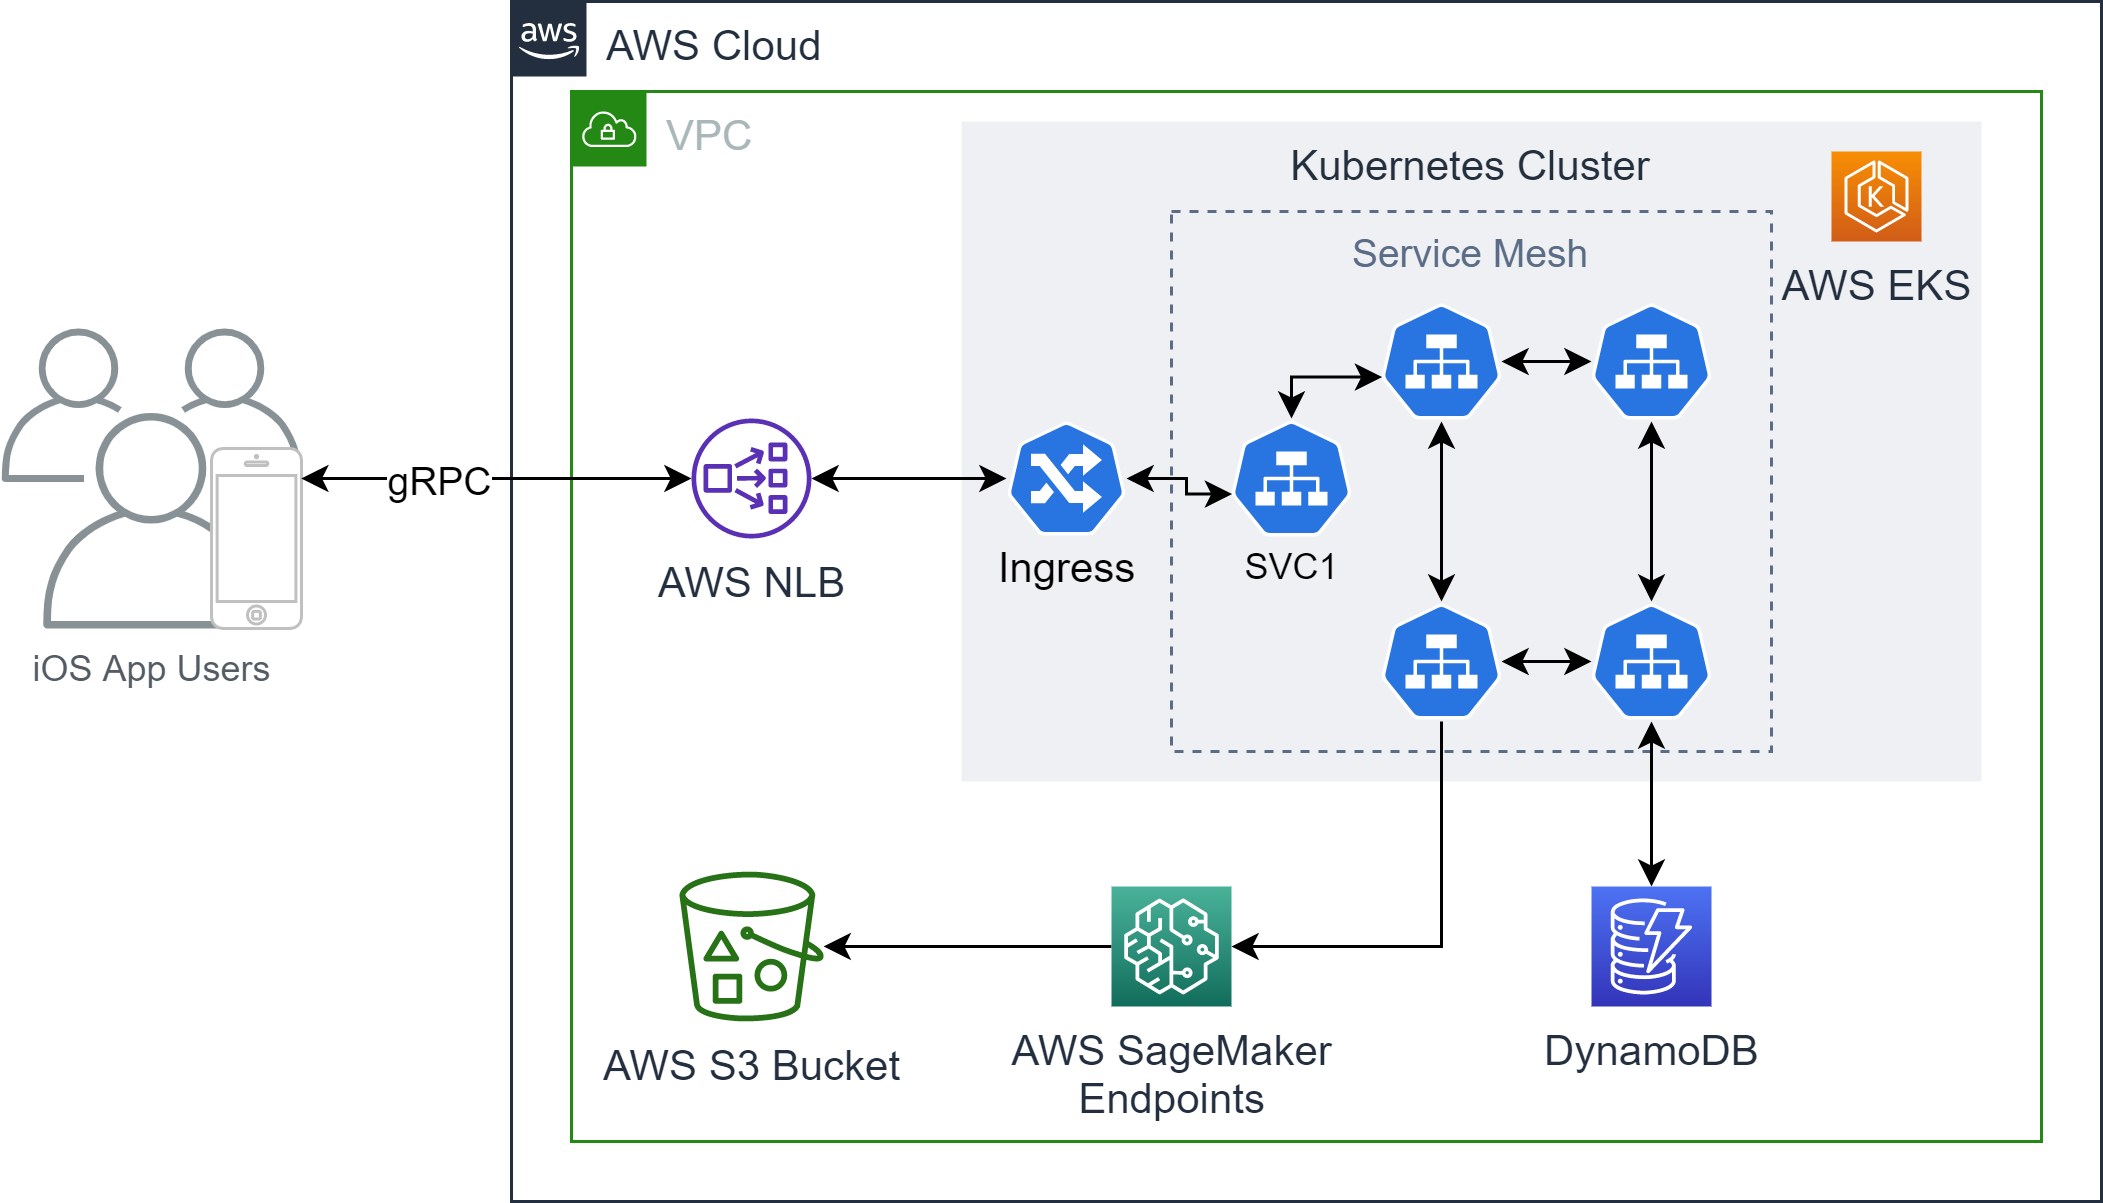
\includegraphics[width=\textwidth]{sphere_arch}
    			\caption{Sphere - Architettura}
    			\label{fig:sphere_arch}
    	    \end{figure}
    	    
    	    I microservizi si dividono in base al linguaggio su cui sono sviluppati, a scelta tra \emph{C++} e \emph{Python 3}, ognuno con le sue dipendenze come descritte nel build system, mentre i moduli mobile si articolano in base alla loro feature, sono scritti interamente in \emph{Swift} e necessitano di ambiente \emph{macOS} per essere compilati. Le interfacce tra i microservizi o tra i moduli mobile e i microservizi sono basate su \emph{gRPC} con formato \emph{ProtoBuf}, mentre tutti i microservizi vengono compilati e pacchettizzati in \emph{container Docker} così da poter seguire il deployment in ambiente \emph{Kubernetes}.
    	
    	\section{Il processo di sviluppo}
    	
    	    \begin{figure}[H]
    			\centering
    			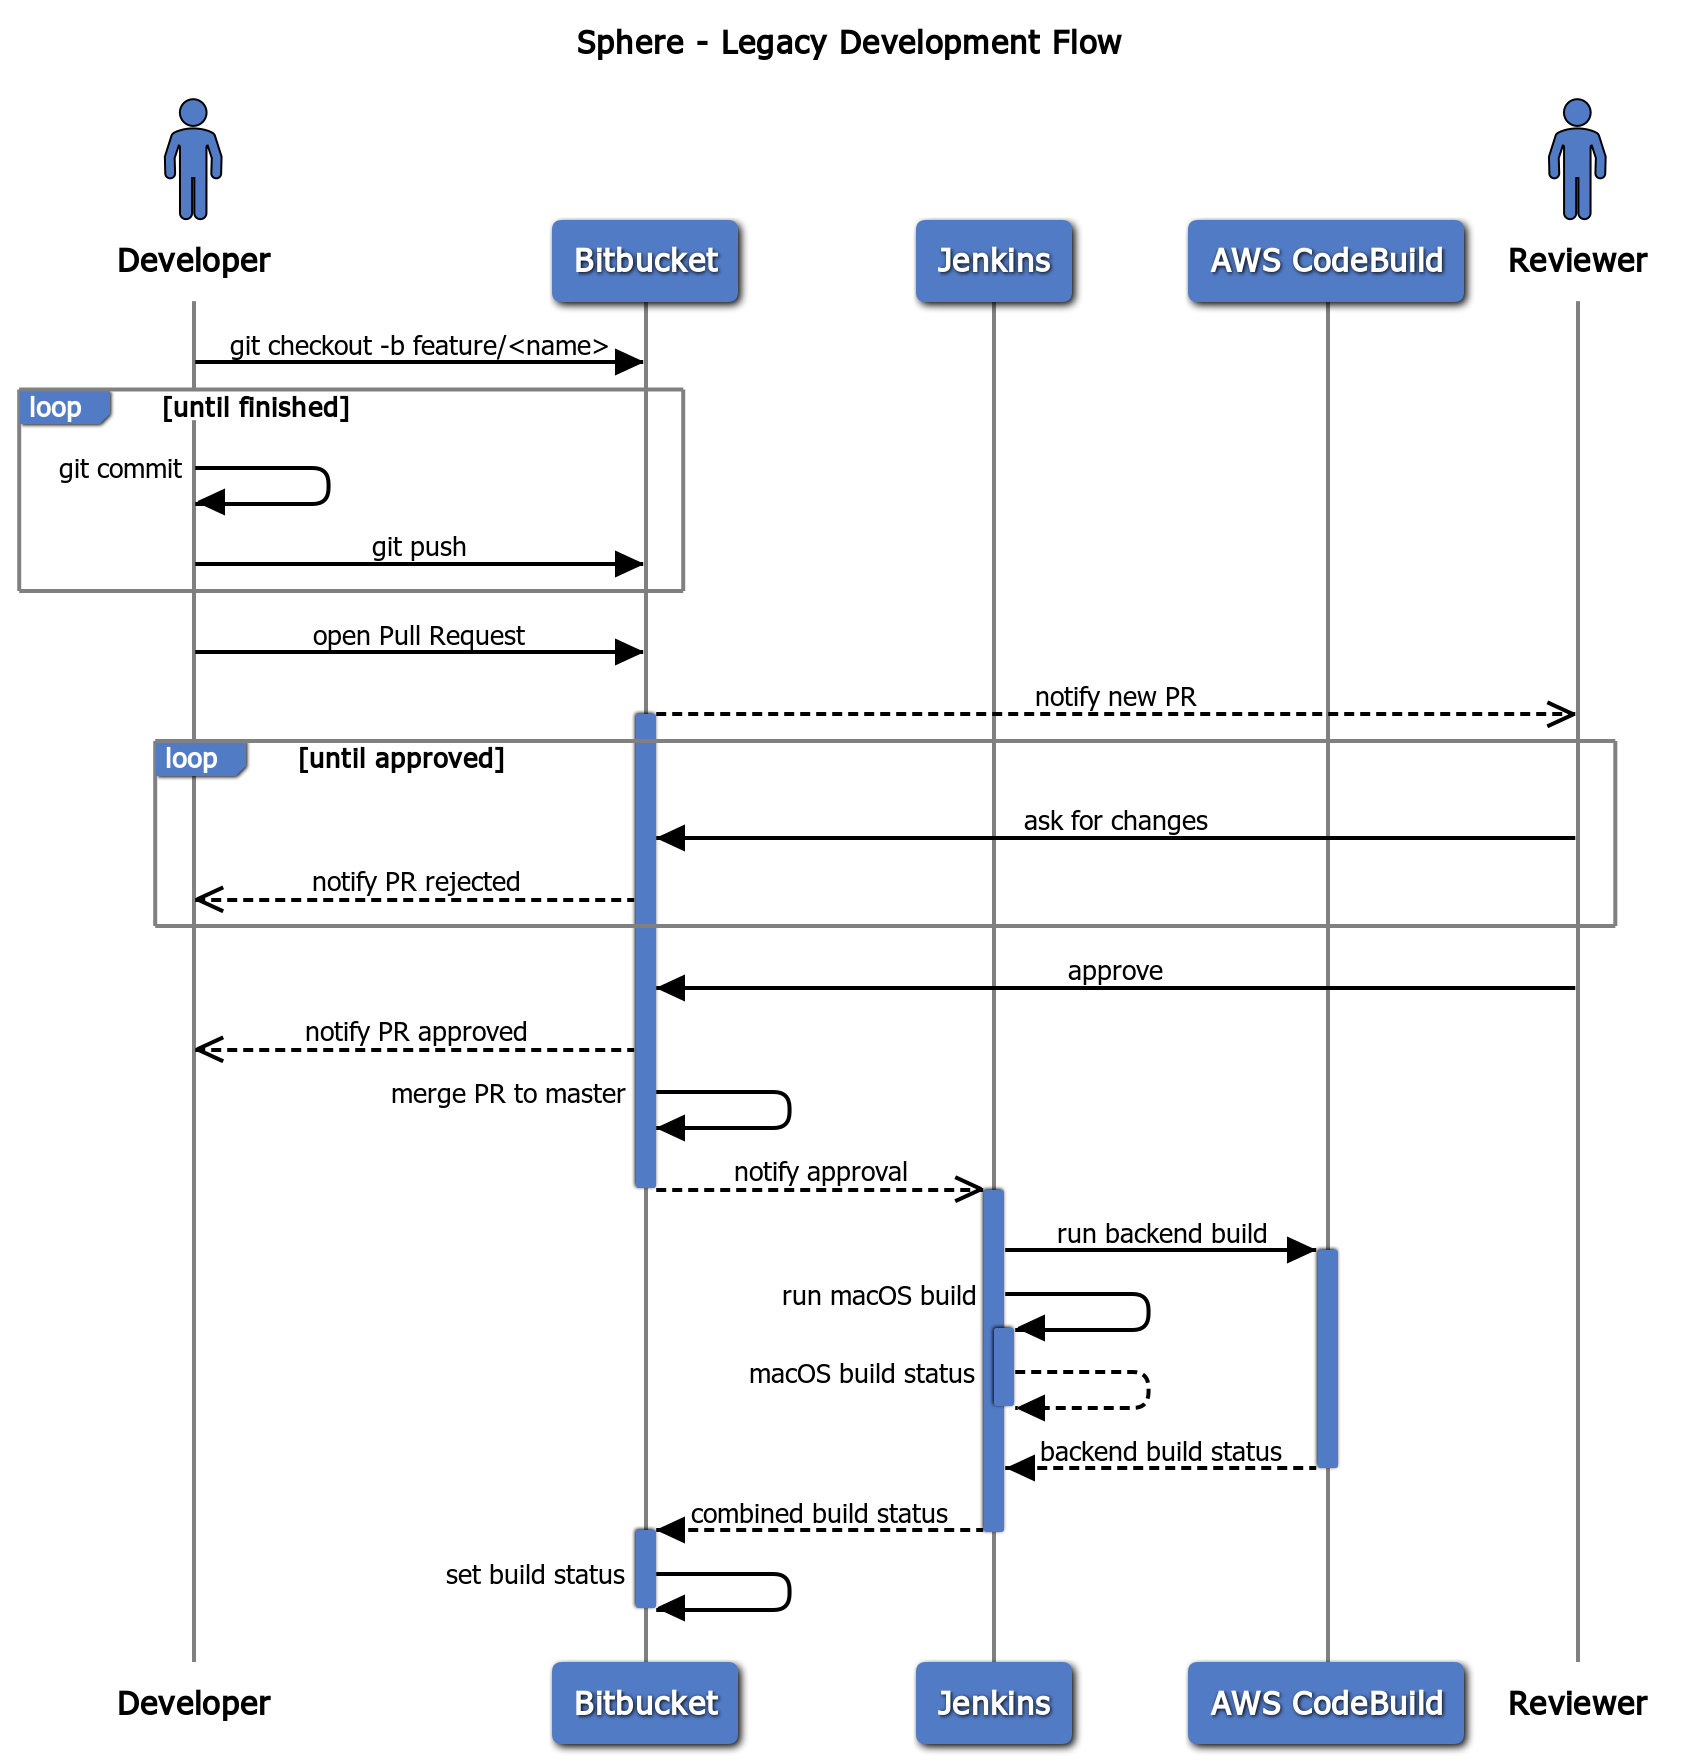
\includegraphics[width=\textwidth]{sphere_legacy_workflow}
    			\caption{Sphere - Workflow Legacy}
    			\label{fig:sphere_legacy_workflow}
    	    \end{figure}
    	    
    	    Il processo in atto prima dell'analisi \emph{DevOps} (figura \ref{fig:sphere_legacy_workflow}) si compone di una gestione a \emph{feature branch}, dove il singolo sviluppatore tiene tutte le sue modifiche rispetto alla \emph{master branch}, ed una volta finito lo sviluppo richiede la code review mediante l'utilizzo di una Pull Request (PR) su Bitbucket.\\*
    	    
    	    L'apertura di una PR scatena una notifica verso il reviewer, senza però interpellare il sistema di \emph{CI} (Jenkins), che viene scatenato solo in fase di accettazione e merge della PR sulla master branch. La \emph{Declarative Pipeline} in atto effettua la build degli artefatti iOS direttamente sulla macchina master (Apple Mac Mini) mentre fa offloading della build dei servizi di backend utilizzando \emph{AWS CodeBuild}, da notare come in nessun caso vengano analizzati i test (unit e integration) e un fallimento avvenga solo ed esclusivamente se la compilazione fallisce.\\*
    	    
    	    Una \textbf{parte mancante} nel processo è di sicuro la \textbf{delivery degli artefatti} prodotti, infatti ne i moduli per iOS ne i servizi di backend vengono compilati e mantenuti in un repository da cui poi attingere in fase di deployment, che viene fatto interamente a mano a seguito di una build manuale, upload manuale e controllo degli artefatti (Docker Containers). Nella nostra analisi non ci concentreremo sulla delivery degli artefatti iOS, su cui è stata applicata una policy differente da parte del team competente.
    	    
    	    Possiamo definire questo processo un primo passo verso un approccio \emph{DevOps}, con diverse mancanze e punti deboli, che andremo a consolidare con l'analisi completa dei requisiti e la creazione di un processo \emph{full DevOps compliant}.
    	
    	\section{Requisiti e KPI}
    	\label{sec:requirements_kpi}
    	
    	    A seguito della analisi del processo preesistente, sono stati formulati dei requisiti funzionali e associati a relativi KPI secondo l'approccio \textbf{SMART} (\emph{Specific, Measurable, Attainable, Relevant, Time-bound}), che il nuovo processo dovrà rispettare per ottenere la qualità attesa e i maggiori benefici:
    	    \begin{itemize}
    	        \item \textbf{\emph{RVisibility}}: il processo dovrà essere sempre disponibile alla consultazione e revisione, anche senza il supporto della infrastruttura on-premise;
                \begin{itemize}
                    \item \textbf{Cloud Readiness} (si/no): gli strumenti utilizzati devono essere disponibili online in ambienti cloud, per migliorare la fruibilità da parte di tutte le utenze;
                \end{itemize}
    	        \item \textbf{\emph{RAvailability}}: il processo dovrà mantenere un livello di \emph{liveness} oltre il 90\% del tempo di utilizzo complessivo, e poter scalare in caso di aumenti di carico;
    	        \begin{itemize}
    	            \item \textbf{Average Availability} (ore per giorno): gli strumenti devono essere sempre disponibili durante tutte le ore di tutti i giorni della settimana, anche se necessitassero di un tempo di \emph{ramp up} minimo;
    	        \end{itemize}
    	        \item \textbf{\emph{REfficiency}}: il processo deve mantenere un livello di efficienza elevato, riducendo al minimo i tempi morti e fornendo agli sviluppatori un sistema sempre pronto all'uso;
    	        \begin{itemize}
    	            \item \textbf{Average Build Time} (in minuti): il processo di \emph{Continuous Integration} deve mantenere un tempo medio di build e testing ragionevole (5 minuti), così da non rallentare l'analisi delle PR da parte dei reviewers;
    	            \item \textbf{Average Build Count} (per giorno): numero di volte che il processo di integrazione/delivery viene utilizzato nell'arco di una giornata lavorativa media;
    	        \end{itemize}
    	        \item \textbf{\emph{RReport}}: il processo dovrà creare un report continuo con l'andamento dello stesso (build, test), per valutare la qualità del codice nel tempo;
    	        \begin{itemize}
    	            \item \textbf{Report Available} (si/no): definisce se il processo ha implementato correttamente un sistema di reportistica per l'andamento delle build e dei test;
    	        \end{itemize}
    	        \item \textbf{\emph{RQuality}}: si dovrà implementare un sistema di code analysis per prevenire il \emph{technical debt} in fasi avanzate di sviluppo;
    	        \begin{itemize}
    	            \item \textbf{QA Available} (si/no): definisce se il processo ha implementato correttamente un sistema di code analysis per quality assurance del codice;
    	        \end{itemize}
    	        \item \textbf{\emph{RTooling}}: utilizzare un tool dedicato a gestire il processo fin dalle primissime fasi, al posto di lasciare l'accesso incondizionato ai repository;
    	        \begin{itemize}
    	            \item \textbf{Unplanned Work Rate} (0-10): il processo deve ridurre al minimo la quantità di lavoro non pianificato, per la sua manutenzione o implementazione di nuove features al suo interno;
    	        \end{itemize}
    	        \item \textbf{\emph{RCost}}: l'infrastruttura a supporto del processo deve contenere i costi il più possibile rispetto al minimo delle risorse necessarie al suo corretto funzionamento;
    	        \begin{itemize}
    	            \item \textbf{Process Cost} (in \$, per run): il costo del processo non deve eccedere il budget allocato aziendalmente.
    	        \end{itemize}
    	    \end{itemize}
    	    
    	%\pagebreak 
    	
	    \section{Analisi del Processo Legacy}
    	    
    	    Prendendo in considerazione il processo descritto precedentemente, ed in atto al momento dell'inizio della fase di transizione verso il nuovo, rileviamo i seguenti dati:
    	    \begin{table}[h]
    	        \centering
    	        \begin{tabular}{ |p{3cm}|p{6cm}||p{2cm}|p{2cm}|  }
                    \hline
                    \textbf{Requirement} & \textbf{KPI Name} & \textbf{KPI Value} & \textbf{Achieved?} \\
                    \hline
                    \emph{RVisibility} & Cloud Readiness & \xmark & \xmark \\
                    \emph{RAvailability} & Average Availability (per day) & 8 hrs & \xmark \\
                    \emph{REfficiency} & Average Build Time & 19 mins & \xmark \\
                    & Average Build Count (per day) & 5 & \xmark \\
                    \emph{RReport} & Report Available & \xmark & \xmark \\
                    \emph{RQuality} & QA Available & \xmark & \xmark \\
                    \emph{RTooling} & Unplanned Work Rate & 4/10 & \cmark \\
                    \emph{RCost} & Process Cost (per run) & 0.4\$ & \cmark \\
                    \hline
                \end{tabular}
    	        \caption{Requisiti e KPIs - Workflow Legacy}
    	        \label{tab:sphere_legacy_kpi}
    	    \end{table}
    	    
    	    Tali dati evidenziano una marcata \textbf{lentezza in fase di compilazione}, con tempistiche molto elevate che costringono gli sviluppatori a notevoli tempi morti di attesa. Come conseguenza dell'utilizzo della CI solo in fase di merge, il \textbf{numero di compilazioni giornaliere è molto basso} e limitato solo al controllo finale nel codice in una fase molto tardiva dello sviluppo. Inoltre, essendo gestito solo ed esclusivamente da una macchina \emph{on-premise}, eventuali cali di tensione, tagli di connessione ad internet o similari possono causare \emph{downtime} inaspettati, necessitando quindi presenza di una persona fisica in ufficio nel caso sorgessero problemi.\\*
    	    
    	    Di pro troviamo un \textbf{rate di lavoro inaspettato relativamente basso}, non essendo stata effettuata particolare manutenzione o aggiornamenti agli strumenti usati, come nemmeno patch di sicurezza, mentre l'unico costo extra rispetto alle risorse on-premise risiede nei tempi di compilazione mediante AWS CodeBuild, che applica un \textbf{costo basso}.
    	   
    	%\pagebreak
    	   
    	\section{Il processo DevOps}
	    \label{sec:devops_process}
    	
    	    Per implementare un processo \emph{DevOps} secondo i requisiti desiderati, si è analizzato il mercato in base alle \emph{Best Practices} utilizzate in ambito enterprise, sondando gli strumenti più utilizzati e rispondenti alle necessità, ed implementando il tutto tenendo in mente un costo contenuto senza perdita di performance.
    	
        	\subsection{Architettura High-Level e Fasi}
        	
        	    Il processo \emph{high-level}, come descritto nell'immagine \ref{fig:sphere_devops_workflow}, si compone di 5 fasi principali:
        	    \begin{enumerate}
        	        \item \textbf{Sviluppo del Codice}: lo sviluppatore, basandosi sulla master branch, scrive il codice localmente fino ad arrivare ad uno stato voluto delle cose;
        	        \item \textbf{Review del Codice}: lo sviluppatore apre una Pull Request (Code Review) mediante un sistema che orchestra il flusso di sviluppo;
        	        \item \textbf{Continuous Integration}: l'orchestratore avvia il testing automatico integrando i cambiamenti nella codebase principale, una volta finito il testing il tool di CI restituisce lo stato dei test che verranno valutati dall'orchestratore. Se le modifiche sono valide, il revisore può decidere di accettare la Pull Request, in caso contrario lo sviluppatore verrà notificato dall'orchestratore del fallimento e sarà chiesto di modificare il codice;
        	        \item \textbf{Accettazione}: il revisore accetta la Pull Request, viene notificato lo sviluppatore e l'orchestratore integra le modifiche nella master branch. Subito dopo, l'orchestratore richiama la \emph{Continuous Integration} per avviare un secondo giro di testing ed analizzare il codice (statico e dinamico), ricavando le metriche qualitative;
        	        \item \textbf{Continuous Delivery}: al momento della release, lo sviluppatore tagga la parte di software da rilasciare mediante una semantica definita, invia il tag al repository di codice che notificherà il processo di \emph{Delivery}. Questo processo creerà gli artefatti software e li distribuirà a sua volta nel repository, seguendo una semantica derivata dal tag iniziale.
        	    \end{enumerate}

        	\subsection{Gestione del Codice}
        	
        	    Il progetto \emph{Sphere}, come accennato nella introduzione del capitolo, si compone di un \emph{monorepo}, ovvero tutti i suoi moduli, dipendenze e librerie vengono gestiti da un singolo repository diviso in sottocartelle e gestito da un build system strutturato.\\*
        	    
        	    Il repository viene hostato su \textbf{Atlassian Bitbucket} mediante backend \textbf{Git}, il sistema \emph{de facto} standard per il code versioning. Nel contesto del flusso \emph{DevOps}, Git viene sfruttato localmente per aprire \emph{feature branches} senza la necessità di mantenerle anche in remoto, e viene sfruttato dall'orchestratore per integrare i cambiamenti effettuati nella codebase principale (master branch).
        	    
           	    \begin{figure}[H]
        			\centering
        			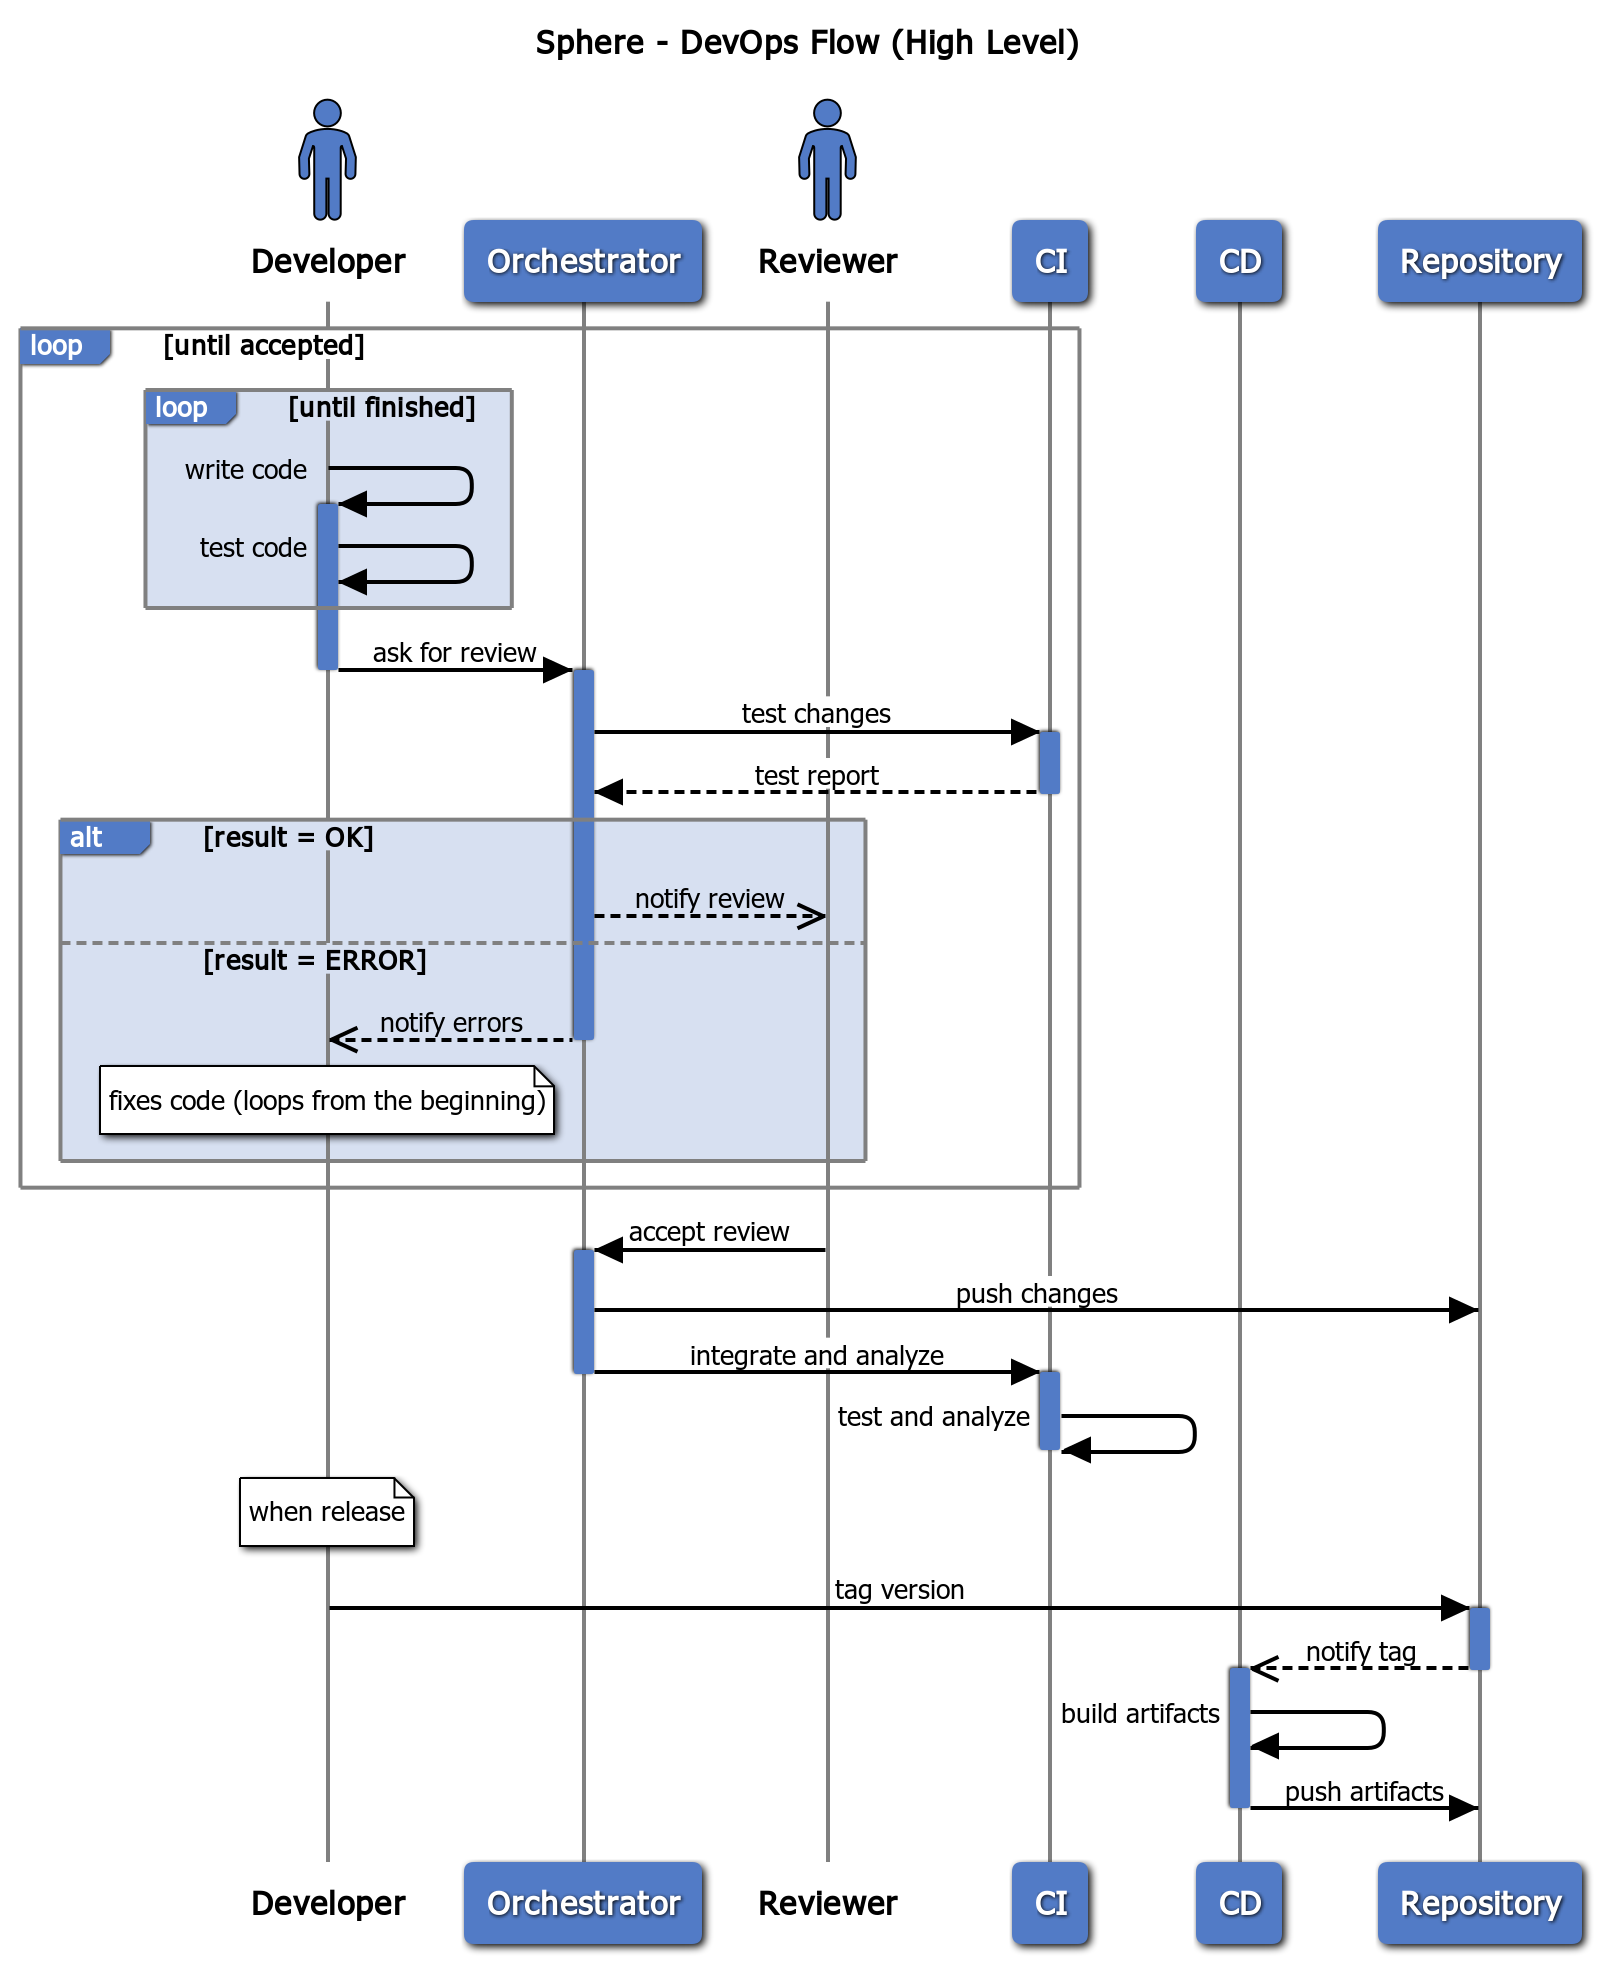
\includegraphics[width=0.9\textwidth]{sphere_devops_workflow}
        			\caption{Sphere - Workflow DevOps}
        			\label{fig:sphere_devops_workflow}
    	        \end{figure}     	
    	        
        	\subsection{Pull Requests e Code Review}
        	
        	    Uno dei capisaldi delle metodologie \emph{Agile} e \emph{DevOps} è la \emph{inspection}, tra cui nasce la pratica che permette di ottenere codice di alta qualità grazie alla sua condivisione con il resto del team, che potrà così visionarlo, commentarlo e fornire feedback continuo sul suo sviluppo. Questo modo di lavorare viene denominato \emph{Code Review}, spesso associata alla \emph{Pull Request}, ovvero la richiesta di "merge" delle modifiche nella codebase principale previa approvazione da parte di uno o più revisori.\\*
        	    
        	    Esistono diversi metodi di Code Review, ma in questa casistica è stato scelto di utilizzare delle Pull Request assistite da uno strumento (l'orchestratore) per permettere a tutti i team di lavorare in modo continuo grazie alla possibilità di poter visionare facilmente le modifiche di una PR, commentarle online collettivamente e fornire feedback sempre efficace.
        	
        	\subsection{Continuous Integration}
    	
    	        La prima fase automatizzata del processo consiste nella pipeline di \emph{Continuous Integration} (CI), gestita da uno strumento dedicato che funge da "motore" ed esegue tutte le sue fasi in base agli input dell'orchestratore. Il suo scopo primario risiede nel controllare tutte le modifiche potenzialmente applicabili dalla accettazione di una Pull Request, integrandole "temporaneamente" nella codebase principale in un ambiente controllato ed avviando il testing o l'analisi del codice in base alla fase del processo.
    	
            	\subsubsection{Test Automation}
            	
            	    Il codice deve essere preparato e scritto in modo da integrare al meglio possibile dei test automatici, sia \textbf{Unit} che \textbf{Integration}, per valutare sia la funzionalità sviluppata che la sua interazione con il resto dei sistemi. Tali test vengono poi avviati dal motore della pipeline di \emph{CI}, risultando in un report contenente lo stato di tutti i test eseguiti, analizzabile da uno strumento esterno o da un revisore.
            	
            	\subsubsection{Code Analysis}
            	
            	    Oltre al testing, il codice può presentare dei potenziali bug, oppure dei code smell che possono sfociare in \emph{technical debt} in un futuro prossimo. Per scongiurare queste cose, viene integrato un sistema di \textbf{analisi statica e dinamica} del codice, interpellato al momento dell'unione delle modifiche con la codebase principale, e che fornisce una valutazione di ciò che si può definire la "qualità" del codice. Le metriche per il quale viene valutata la qualità sono configurabili in base alle esigenze del progetto, così da non risultare troppo banali o troppo restrittive.
    	
    	    \subsection{Continuous Delivery}
    	    
    	        L'ultima fase automatizzata del processo consiste nella pipeline di \emph{Continuous Delivery}, gestita spesso dallo stesso motore della \emph{CI}, permette di compilare, pacchettizzare e raccogliere tutti gli artefatti software pronti per una release da effettuare o per utilizzi futuri. Nel processo definito, questo processo viene utilizzato \emph{on demand} in base alla pianificazione delle release, e richiamabile su singoli moduli del progetto.
    	
            	\subsubsection{Build Automation}
            	
            	    Grazie alla integrazione della codebase con un \emph{Build System} unificato, risulta molto semplice effettuare automazione della compilazione dei singoli artefatti, in base ad uno specifico \textbf{target} definito in fase di richiesta della delivery. La compilazione avviene inoltre in un ambiente controllato e definito a priori, sempre uguale e riproducibili, riducendo così eventuali variabili in gioco che possono compromettere la qualità del prodotto finale.
            	
            	\subsubsection{Artifacts Delivery}
            	    
            	    Gli artefatti software prodotti mediante compilazione vengono poi pacchettizzati come \emph{Containers} ed inviati ad un repository (registry) per storage ed utilizzi futuri in un ipotetico deploy in un ambiente scelto.
    	
        	\subsection{Deployment}
        	
        	    Dalla descrizione del processo high-level si è esclusa l'analisi della fase di Deployment, essendo una questione legata molto al modello di business attuale, che non vede l'azienda come fornitore del servizio in se ma solo fornitore della tecnologia. Vi sono quindi gli ambienti di testing gestiti internamente, il cui deployment viene effettuato \textbf{manualmente} in base alle esigenze, facilitato dall'utilizzo di tecnologie come \emph{Container Orchestration} mediante \emph{Kubernetes}.
    	
    	\section{Tecnologie e Strumenti}
    	
        	\subsection{SCM: Git}
        	
        	    Originariamente sviluppato da \emph{Linus Torvalds}, \emph{Git}\cite{git} si propone come un tool estremamente performante con la caratteristica di essere distribuito e non centralizzato, quindi ogni sviluppatore può mantenere una copia del codice localmente e lavorare senza necessità di essere collegato ad un repository centrale. La sua struttura permette di gestire efficacemente flussi complessi e strutture dati complesse, oltre che permettere lo storage di grandi file utilizzando \textbf{Git-LFS} (\emph{Large File Storage}). Git è stato scelto inoltre per la sua compatibilità con Atlassian Bitbucket, e per il suo utilizzo estremamente diffuso.
    	
        	\subsection{Build System: Bazel}
        	
        	    Progetto nato dal tool interno di \emph{Google} chiamato \emph{Blaze}, \textbf{Bazel}\cite{bazel} è un build system che supporta progetti di grandi dimensioni in molteplici linguaggi, fornisce un linguaggio high-level per descrivere gli artefatti, le configurazioni e le dipendenze dei moduli da compilare, ed è multipiattaforma.\\*
        	    
        	    Bazel mantiene una \textbf{cache interna} di tutti gli artefatti compilati precedentemente, ricompilando solo quelli che necessitano di cambiamenti e velocizzando i tempi notevolmente, permette inoltre di utilizzare una cache remota condivisa tra i vari sistemi dove viene eseguito. Ad ogni sua esecuzione, leggendo i file descrittori di compilazione, crea un \textbf{Action Graph} che definisce tutte le azioni da eseguire e le dipendenze tra i vari moduli o artefatti, permettendo build sempre corrette, ermetiche e riproducibili.
    	
        	\subsection{Cloud Provider: AWS}
        	
        	    \textbf{Amazon Web Services} (abbreviato \emph{AWS}) è una sussidiaria del colosso dell'ecommerce \emph{Amazon}, e si propone come il più grande \emph{cloud provider} attualmente sul mercato con oltre 46 miliardi di dollari di fatturato annuo in costante crescita. I servizi proposti spaziano dall'\emph{IaaS}, al \emph{PaaS} fino al \emph{SaaS}, mantenendo però forte vantaggio in ambito infrastruttura e servizi managed. AWS è stato scelto a livello progettuale per la sua potenza, flessibilità e competitività sul mercato.
    	
        	\subsection{Orchestrator: Phabricator ed Arcanist}
    	
    	        Nato da un progetto interno a \emph{Facebook}, il suo lead developer Evan Priestley ha poi lasciato l'azienda per continuare il suo sviluppo esternamente fondando \emph{Phacility}, \textbf{Phabricator}\cite{phabricator} è un multi-tool di \emph{development collaboration} che integra diversi strumenti utili in un meccanismo di sviluppo \emph{Agile-oriented}.
    	        
    	        \begin{figure}[H]
        			\centering
        			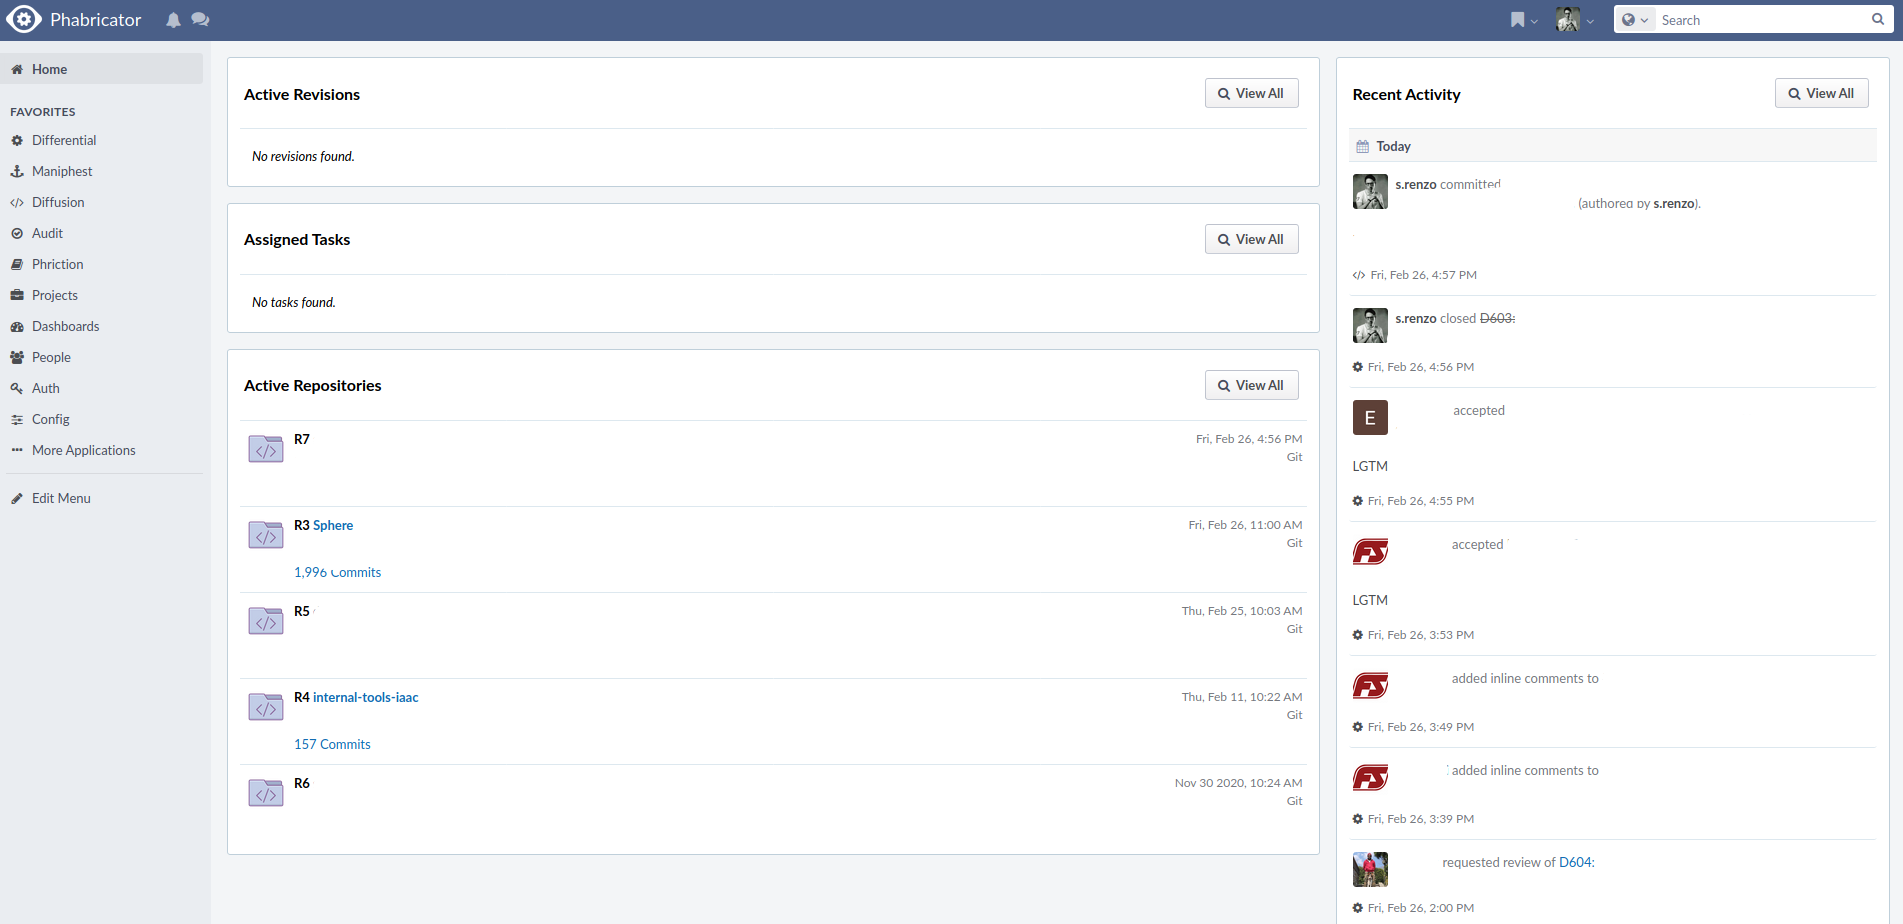
\includegraphics[width=0.9\textwidth]{phabricator}
        			\caption{Phabricator Web UI}
        			\label{fig:phabricator}
    	        \end{figure}
    	        
    	        Nel progetto verrà sfruttato \emph{Differential}, il sistema di Pull Requests e Code Review, e \emph{Diffusion} che permette di integrare lo strumento con repository Git (anche remoti). Verrà inoltre descritto l'uso di \textbf{Arcanist}, strumento di \emph{CLI} (Command Line Interface) che semplifica l'interazione con Phabricator e l'implementazione del flusso di sviluppo voluto.
    	
        	\subsection{CI/CD: Jenkins}
        	
        	    Come sistema di automazione \emph{CI/CD} è stato scelto \textbf{Jenkins}\cite{jenkins}, software basato su Java in ambiente Apache Tomcat, \emph{de facto} uno dei tool più utilizzati al mondo in fatto di pipeline di automazione, e che offre una interfaccia web semplice da utilizzare,  illustrata nell'immagine \ref{fig:jenkins_ui}.\\*
        	    
        	    Jenkins trova la sua forza nella flessibilità di utilizzo ed estensibilità, mediante vari tipi di oggetti creabili e gestibili e l'installazione di una miriade di \emph{plugins} mantenuti sia ufficialmente che dalla comunità open source. Lo strumento permette inoltre di fare \emph{offloading} di alcuni task verso macchine remote gestite dallo stesso, mediante il sistema degli \textbf{agents}.
    	
    	    \subsection{Code Analysis: SonarQube}
    	    
    	        Il sistema di \emph{static e dynamic code analysis} scelto è \textbf{SonarQube}, strumento molto diffuso e open source, che permette di analizzare, quantificare e fare reporting di metriche di qualità del codice in base a regole e soglie ben definite da un "profilo" di qualità, e che fornisce una web UI per visionare tali analisi, illustrata in figura \ref{fig:sonarqube_ui}.\\*
    	        
    	        SonarQube permette di analizzare potenziali bug, code smells, codice duplicato o poco testato, con delle semplici configurazioni e tool di supporto come \textbf{Sonar Scanner} che interagiscono col sistema centrale facilitando le analisi.
    	        
    	        \begin{figure}[H]
        			\centering
        			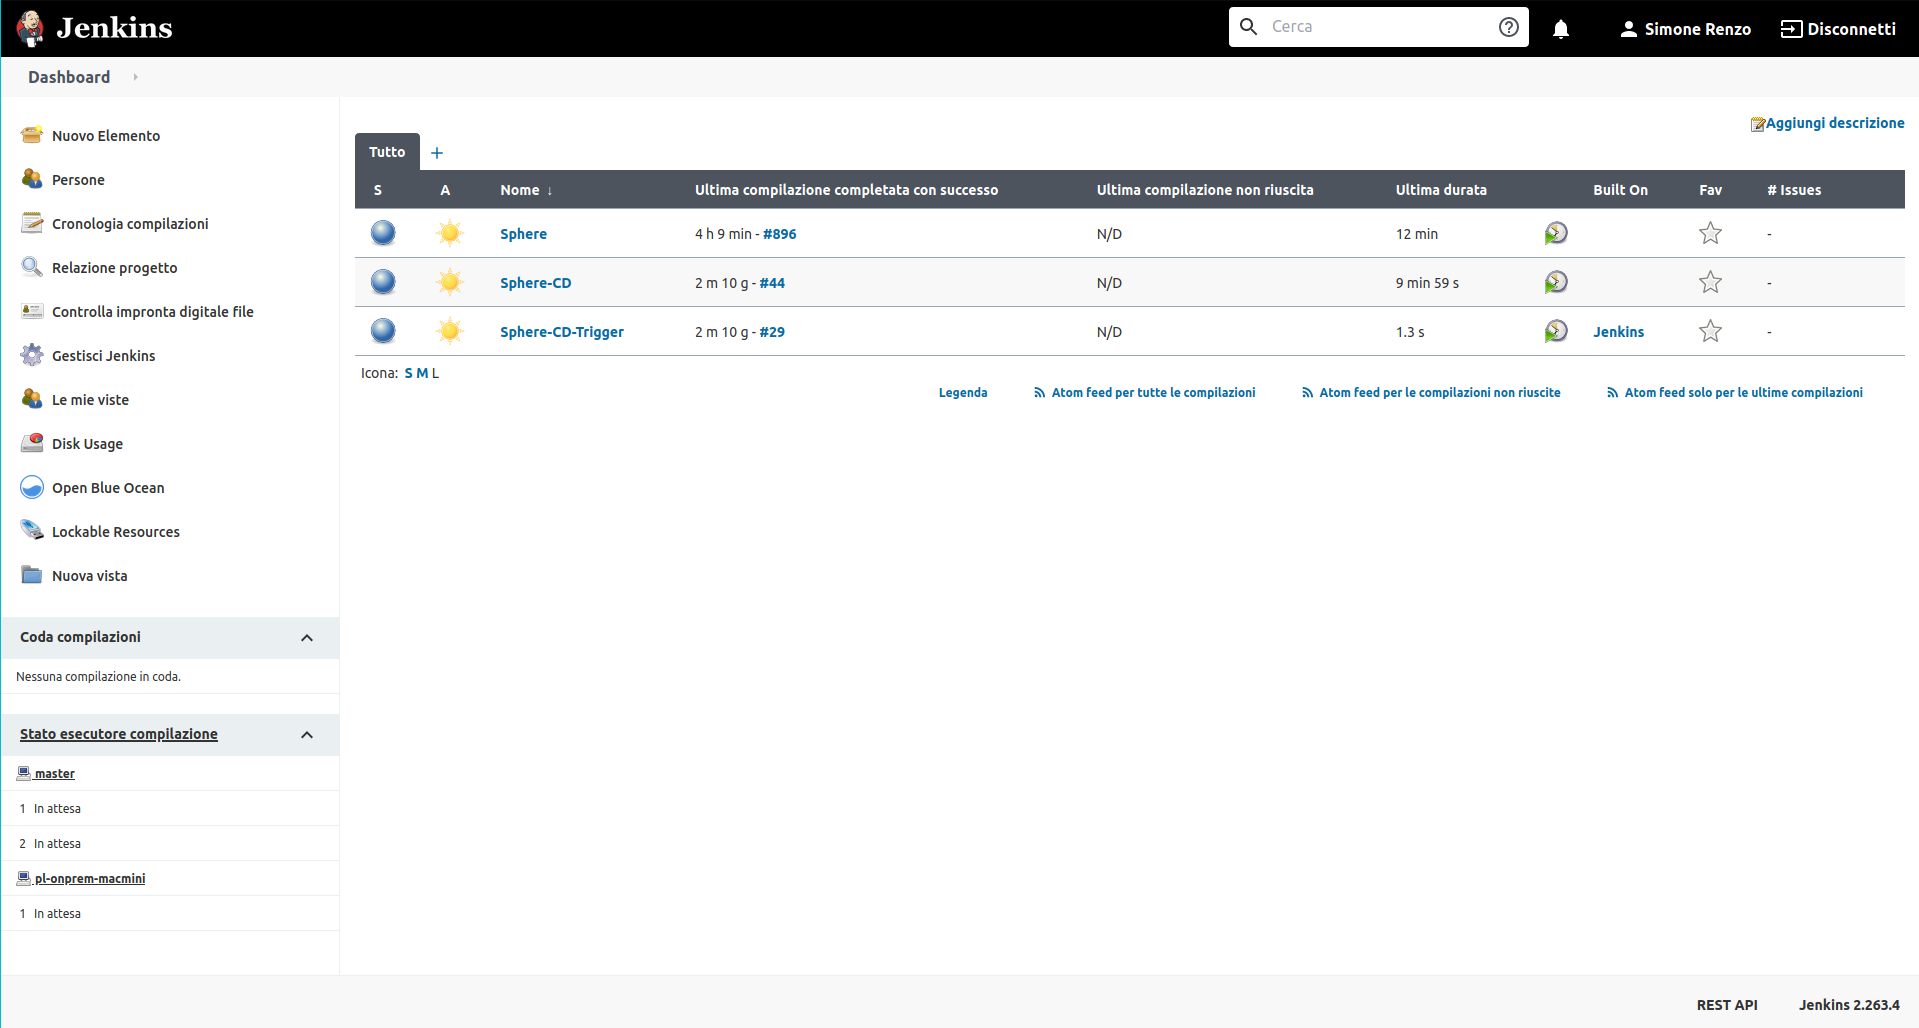
\includegraphics[width=0.9\textwidth]{jenkins}
        			\caption{Jenkins Web UI}
        			\label{fig:jenkins_ui}
    	        \end{figure}
    	        
    	        \begin{figure}[H]
        			\centering
        			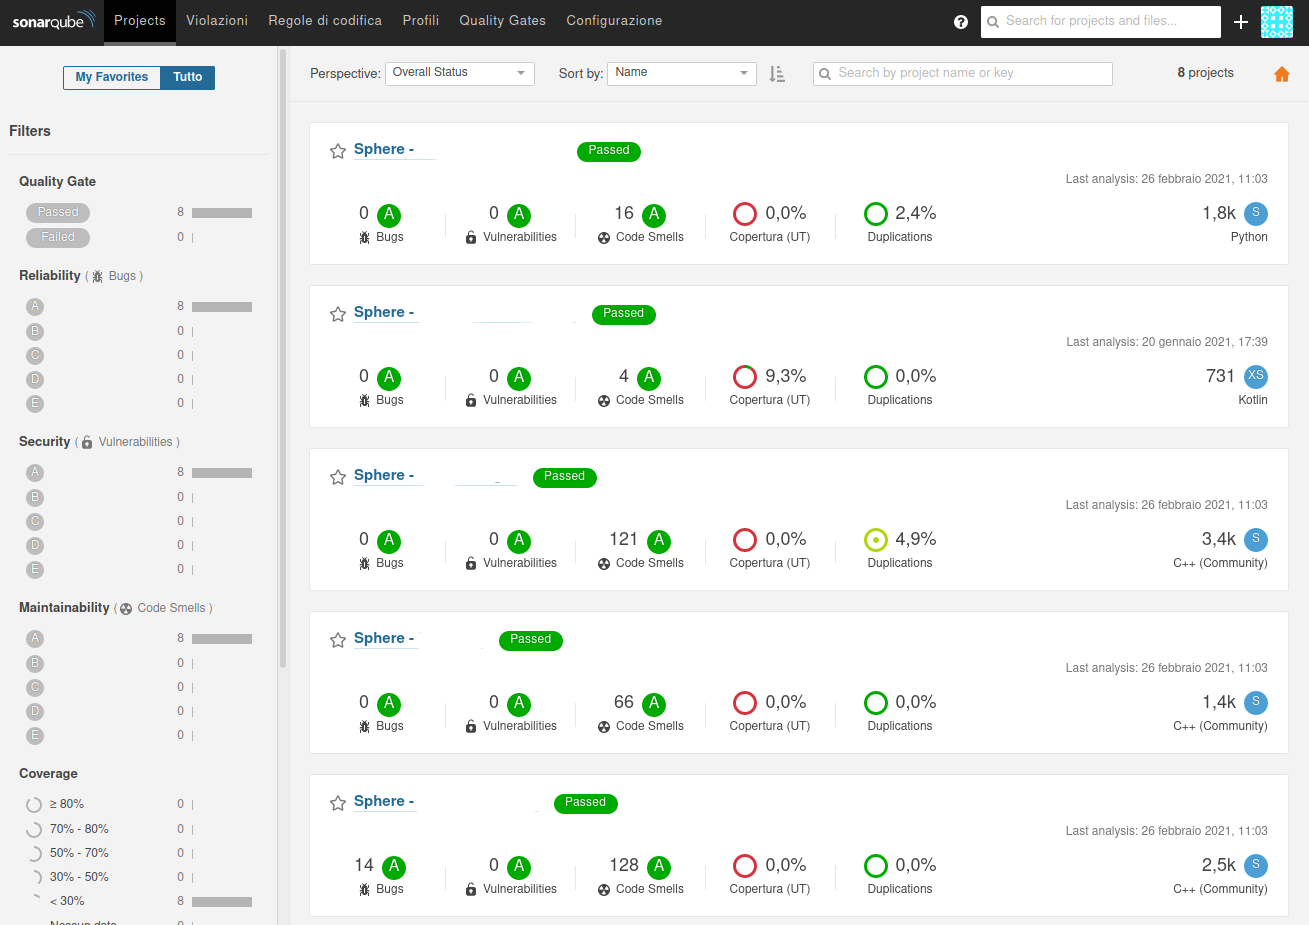
\includegraphics[width=0.9\textwidth]{sonarqube}
        			\caption{SonarQube Web UI}
        			\label{fig:sonarqube_ui}
    	        \end{figure}
    	        
    \section{Analisi del Processo \emph{DevOps}}
    
        A seguito della descrizione, implementazione ed utilizzo del processo \emph{DevOps} high level, si necessita la valutazione dei vari aspetti come descritti dai \hyperref[sec:requirements_kpi]{Requisiti e KPI}:
        \begin{table}[H]
	        \centering
	        \begin{tabular}{ |p{3cm}|p{6cm}||p{2cm}|p{2cm}||p{1.5cm}|  }
                \hline
                \textbf{Requirement} & \textbf{KPI Name} & \textbf{KPI Value} & \textbf{Achieved?} & \textbf{Gain} \\
                \hline
                \emph{RVisibility} & Cloud Readiness & \cmark & \cmark & +100\% \\
                \emph{RAvailability} & Average Availability (per day) & 24 hrs & \cmark & +67\% \\
                \emph{REfficiency} & Average Build Time & 4 mins & \cmark & -375\% \\
                & Average Build Count (per day) & 15 & \cmark & +67\% \\
                \emph{RReport} & Report Available & \cmark & \cmark & +100\% \\
                \emph{RQuality} & QA Available & \cmark & \cmark & +100\% \\
                \emph{RTooling} & Unplanned Work Rate & 2/10 & \cmark & -50\% \\
                \emph{RCost} & Process Cost (per run) & 2.6\$ & \cmark & +84\% \\
                \hline
            \end{tabular}
	        \caption{Requisiti e KPIs - Workflow DevOps}
	        \label{tab:sphere_devops_kpi}
	    \end{table}
	    
	    Possiamo notare il notevole \textbf{guadagno} in merito di \textbf{tempo di compilazione} e \textbf{numero di compilazioni} giornaliere, sintomo che il processo implementato permette di ridurre i tempi morti degli sviluppatori ed ottimizzare al meglio il \emph{throughput} massimo. Il processo aggiunge inoltre un sistema di \emph{report} visibile a tutti, gestito dagli strumenti in base al loro scopo, assieme ad un tool di \emph{Quality Assurance} del codice (code analysis) che permette di ridurre il debito tecnico nel tempo se affrontato nel modo corretto. Altro punto a favore è sicuramente la \textbf{cloud readiness} dell'intero deployment, che permette di essere ricreato in pochissimo tempo e riprodotto all'infinito.\\*
	    
	    L'unico reale punto negativo, seguendo le metriche definite, è il \textbf{costo} del processo per ogni volta che viene sfruttato. Questo deriva dalle \textbf{risorse Cloud} necessarie a mantenere attivi gli strumenti scelti e sempre disponibili da parte degli sviluppatori, oltre che dall'accesso alle risorse mediante rete protetta (VPN). Ovviamente questa nuova infrastruttura permette di ottenere una manutenzione meno indispensabile, se non con mirati aggiornamenti di sicurezza o \emph{features} ove necessarie, sempre effettuate grazie all'utilizzo dei tool di \emph{IaC} e \emph{CaC}.

\end{document}